%% abtex2-modelo-trabalho-academico.tex, v-1.9.6 laurocesar
%% Copyright 2012-2016 by abnTeX2 group at http://www.abntex.net.br/ 
%%
%% This work may be distributed and/or modified under the
%% conditions of the LaTeX Project Public License, either version 1.3
%% of this license or (at your option) any later version.
%% The latest version of this license is in
%%   http://www.latex-project.org/lppl.txt
%% and version 1.3 or later is part of all distributions of LaTeX
%% version 2005/12/01 or later.
%%
%% This work has the LPPL maintenance status `maintained'.
%% 
%% The Current Maintainer of this work is the abnTeX2 team, led
%% by Lauro César Araujo. Further information are available on 
%% http://www.abntex.net.br/
%%
%% This work consists of the files abntex2-modelo-trabalho-academico.tex,
%% abntex2-modelo-include-comandos and abntex2-modelo-references.bib
%%

% ------------------------------------------------------------------------
% ------------------------------------------------------------------------
% abnTeX2: Modelo de Trabalho Academico (tese de doutorado, dissertacao de
% mestrado e trabalhos monograficos em geral) em conformidade com 
% ABNT NBR 14724:2011: Informacao e documentacao - Trabalhos academicos -
% Apresentacao
% ------------------------------------------------------------------------
% ------------------------------------------------------------------------


\documentclass[
  10.5pt,				  % tamanho da fonte
	openright,			% capítulos começam em pág ímpar (insere página vazia caso preciso)
	twoside,			  % para impressão em recto e verso. Oposto a oneside  
  a5paper,
  chapter=TITLE,	% títulos de capítulos convertidos em letras maiúsculas
	section=TITLE,	% títulos de seções convertidos em letras maiúsculas
  hyphens,        % faz a quebra de linhas em URLs muito longas
	% -- opções do pacote babel --
	english,        % idioma adicional para hifenização
	brazil          % o último idioma é o principal do documento
]{abntex2}

% ---
% Pacotes básicos 
% ---
\usepackage{lmodern}          % Usa a fonte Latin Modern			
\usepackage[T1]{fontenc}      % Selecao de codigos de fonte.
\usepackage[utf8]{inputenc}	  % Codificacao do documento (conversão automática dos acentos)
\usepackage{lastpage}         % Usado pela Ficha catalográfica
\usepackage{indentfirst}      % Indenta o primeiro parágrafo de cada seção.
\usepackage{color}				    % Controle das cores
\usepackage{graphicx}			    % Inclusão de gráficos
\usepackage{microtype} 			  % Para melhorias de justificação
\usepackage[final]{pdfpages}
\usepackage{listings}         % Para incluir código fonte com formatação

%\usepackage{multirow}         % Permite a mesclagem de linhas em tabelas
%\usepackage{adjustbox}        % Permite o escalonamento do conteúdo que não cabe em uma página
%\usepackage{tabularx}         % Impede o overflow de tabelas. 
%\usepackage{rotating}         % Rotaciona tabelas.
%\usepackage{placeins}         % Permite usar \FloatBarrier

% ---

% ---
% Pacotes adicionais, usados apenas no âmbito do Modelo Canônico do abnteX2
% ---
\usepackage{lipsum}				% para geração de dummy text
%\usepackage{cmap}
% ---

% ---
% Lista de símbolos e acrônimos
% ---
%\usepackage{abntex2glossaries}  % Deve ser incluído antes de abntex2cite

% ---
% Pacotes de citações
% ---
\usepackage[brazilian,hyperpageref]{backref} % Paginas com as citações na bibl
%\usepackage[alf]{abntex2cite}	              % Citações utilizando o padrão autor-data de chamadas
\usepackage[num,overcite]{abntex2cite}       % Citações utilizando o padrão numérico de chamadas
\citebrackets()


% --- 
% CONFIGURAÇÕES DE PACOTES
% --- 

% ---
% Configurações do pacote backref
% Usado sem a opção hyperpageref de backref
\renewcommand{\backrefpagesname}{Citado na(s) página(s):~}
% Texto padrão antes do número das páginas
\renewcommand{\backref}{}
% Define os textos da citação
\renewcommand*{\backrefalt}[4]{
	\ifcase #1 %
		Nenhuma citação no texto.%
	\or
		Citado na página #2.%
	\else
		Citado #1 vezes nas páginas #2.%
	\fi}%
% ---

% ---
% Correção das margens
% ---
\setlrmarginsandblock{2.5cm}{1.5cm}{*}
\setulmarginsandblock{2.0cm}{1.5cm}{*}
\checkandfixthelayout
% ---
% Correção das fontes das seções
% ---
\renewcommand{\ABNTEXchapterfont}{\fontfamily{lm}\fontseries{b}\selectfont}
\renewcommand{\ABNTEXchapterfontsize}{\normalsize}
\renewcommand{\ABNTEXsectionfont}{\ABNTEXchapterfont}
\renewcommand{\ABNTEXsectionfontsize}{\normalsize}
\renewcommand{\ABNTEXsubsectionfont}{\ABNTEXchapterfont}
\renewcommand{\ABNTEXsubsectionfontsize}{\normalsize}
\renewcommand{\ABNTEXsubsubsectionfont}{\ABNTEXchapterfont}
\renewcommand{\ABNTEXsubsubsectionfontsize}{\normalsize}
% ---
% Correção do espaçamento no primeiro parágrafo
% ---
\setlength\afterchapskip{\lineskip}
% ---
% Caminho para as imagens
% ---
\graphicspath{{./img/}}
% ---
% Listings
% ---
\renewcommand{\lstlistingname}{Algoritmo}% Listing -> Algoritmo
\renewcommand{\lstlistlistingname}{Lista de \lstlistingname s}% List of Listings -> Lista de Algoritmos
\definecolor{mygreen}{rgb}{0,0.6,0}
\definecolor{mygray}{rgb}{0.5,0.5,0.5}
\definecolor{mymauve}{rgb}{0.58,0,0.82}
\lstset{ %
  backgroundcolor=\color{white},   % choose the background color;
  basicstyle=\footnotesize,        % the size of the fonts that are used for the code
  breakatwhitespace=false,         % sets if automatic breaks should only happen at whitespace
  breaklines=true,                 % sets automatic line breaking
  captionpos=t,                    % sets the caption-position to bottom
  commentstyle=\color{mygreen},    % comment style
  deletekeywords={...},            % if you want to delete keywords from the given language
  escapeinside={\%*}{*)},          % if you want to add LaTeX within your code
  extendedchars=true,              % lets you use non-ASCII characters; for 8-bits encodings only, does not work with UTF-8
  frame=single,	                   % adds a frame around the code
  keepspaces=true,                 % keeps spaces in text, useful for keeping indentation of code (possibly needs columns=flexible)
  keywordstyle=\color{blue},       % keyword style
  language=Java,                   % the language of the code
  morekeywords={*,...},            % if you want to add more keywords to the set
  numbers=none,                    % where to put the line-numbers; possible values are (none, left, right)
  numbersep=5pt,                   % how far the line-numbers are from the code
  numberstyle=\tiny\color{mygray}, % the style that is used for the line-numbers
  rulecolor=\color{black},         % if not set, the frame-color may be changed on line-breaks within not-black text (e.g. comments (green here))
  showspaces=false,                % show spaces everywhere adding particular underscores; it overrides 'showstringspaces'
  showstringspaces=false,          % underline spaces within strings only
  showtabs=false,                  % show tabs within strings adding particular underscores
  stepnumber=2,                    % the step between two line-numbers. If it's 1, each line will be numbered
  stringstyle=\color{mymauve},     % string literal style
  tabsize=2,	                     % sets default tabsize to 2 spaces
  title=\lstname,                  % show the filename of files included with \lstinputlisting; also try caption instead of title
  numberbychapter=false            % number lists by chapter or sequentially from the beginning of the document
}

% ----------------------------------------------------------
% PREÂMBULO
% ----------------------------------------------------------

\titulo{Atualização Tecnológica do Formulário de Inscrição do Processo Seletivo da Pós-Graduação da UFSC}
\autor{Makhles Reuter Lange}
\data{\today}
%\instituicao{Universidade Federal de Santa Catarina}
\instituicao{%
  Universidade Federal de Santa Catarina - UFSC
  \par
  Ciência da Computação}
\local{Florianópolis}
\tipotrabalho{Exemplo para referência futura}
\orientador{Andréia Alves dos Santos Schwaab}
\coorientador{Leandro José Komosinski}
\tipotrabalho{Trabalho de Conclusão de Curso}
\preambulo{Trabalho de Conclusão de Curso submetido ao Curso de Ciências da Computação da Universidade Federal de Santa Catarina para a obtenção do grau de Bacherel em Ciências da Computação.}

% ---
% Configurações de aparência do PDF final

% alterando o aspecto da cor azul
\definecolor{blue}{RGB}{41,5,195}

% informações do PDF
\makeatletter
\hypersetup{
     	%pagebackref=true,
		pdftitle={\@title}, 
		pdfauthor={\@author},
    	pdfsubject={\imprimirpreambulo},
	    pdfcreator={TeXmaker},
		pdfkeywords={tcc}{latex}{primefaces}{java}{jsf}{trabalho acadêmico}, 
		colorlinks=true,       		% false: boxed links; true: colored links
    	linkcolor=blue,          	% color of internal links
    	citecolor=blue,        		% color of links to bibliography
    	filecolor=magenta,      		% color of file links
		urlcolor=blue,
		bookmarksdepth=4
}
\makeatother
% --- 

% --- 
% Espaçamentos entre linhas e parágrafos 
% --- 

% O tamanho do parágrafo é dado por:
\setlength{\parindent}{1.0cm}

% Controle do espaçamento entre um parágrafo e outro:
\setlength{\parskip}{0.2cm}  % tente também \onelineskip

\begin{document}

% Seleciona o idioma do documento (conforme pacotes do babel)
%\selectlanguage{english}
\selectlanguage{brazil}

% Retira espaço extra obsoleto entre as frases.
\frenchspacing


% ----------------------------------------------------------
% ELEMENTOS PRÉ-TEXTUAIS
% ----------------------------------------------------------
\pretextual%
% ---
% Capa
% ---
\imprimircapa%
% ---
% Folha de rosto
% (o * indica que haverá a ficha bibliográfica)
% ---
\imprimirfolhaderosto*%
% ---
\clearpage
%\imprimirfichacatalografica%
%\clearpage

% ----------------------------------------------------------
% FOLHA DE APROVAÇÃO
% ----------------------------------------------------------

% Isto é um exemplo de Folha de aprovação, elemento obrigatório da NBR
% 14724/2011 (seção 4.2.1.3). Você pode utilizar este modelo até a aprovação
% do trabalho. Após isso, substitua todo o conteúdo deste arquivo por uma
% imagem da página assinada pela banca com o comando abaixo:
%
%\includepdf{folhadeaprovacaoassinada.pdf}
%
\begin{folhadeaprovacao}

  \begin{center}
    {\ABNTEXchapterfont\large\imprimirautor}

    \vspace*{\fill}\vspace*{\fill}
    \begin{center}
      \ABNTEXchapterfont\bfseries\Large\imprimirtitulo
    \end{center}
    \vspace*{\fill}
    
    \hspace{.45\textwidth}
    \begin{minipage}{.5\textwidth}
        \imprimirpreambulo
    \end{minipage}%
    \vspace*{\fill}
   \end{center}
        
   Trabalho aprovado. \imprimirlocal, \imprimirdata:

   \assinatura{\textbf{\imprimirorientador} \\ Orientador} 
   \assinatura{\textbf{\imprimircoorientador} \\ Coorientador}
   \assinatura{\textbf{Beatriz Wilges} \\ Convidado 1}
   \assinatura{\textbf{Verônica de Souza de Melo} \\ Convidado 2}

   \begin{comment}
  \begin{center}
    \vspace*{0.5cm}
    {\large\imprimirlocal}
    \par
    {\large\imprimirdata}
    \vspace*{1cm}
  \end{center}
  \end{comment}
\end{folhadeaprovacao}


% ----------------------------------------------------------
% RESUMOS
% ----------------------------------------------------------

\begin{resumo}
Texto do resumo.
\vspace{\onelineskip} \\
\noindent \textbf{Palavras-chave:} Formulário de Inscrição; Processo Seletivo; JavaServer Faces; Primefaces;
\end{resumo}
% ---
\begin{resumo}[Abstract]
\begin{otherlanguage*}{english}
The abstract.
\vspace{\onelineskip} \\
\noindent \textbf{Keywords:} Application Form; Selective Process; JavaServer Faces; Primefaces;
\end{otherlanguage*}
\end{resumo}


% ---
% Lista de ilustrações
% ---
%\pdfbookmark[0]{\listfigurename}{lof}
%\listoffigures*
%\cleardoublepage
% ---

% ---
% Lista de tabelas
% ---
%\pdfbookmark[0]{\listtablename}{lot}
%\listoftables*
%\cleardoublepage
% ---

% ---
% Lista de abreviaturas e siglas
% ---
\begin{siglas}
  \item[Java EE] Java Enterprise Edition
  \item[JSF]     JavaServer Faces
  \item[JPA]     Java Persistence API
  \item[SeTIC]   Superintendência de Governança Eletrônica e Tecnologia da Informação e Comunicação
\end{siglas}



% ----------------------------------------------------------
% SUMÁRIO
% ----------------------------------------------------------
\pdfbookmark[0]{\contentsname}{toc}
\tableofcontents*
\cleardoublepage
% ---



% ----------------------------------------------------------
% ELEMENTOS TEXTUAIS
% ----------------------------------------------------------
\textual%




\chapter{Introdução}
% ----------------------------------------------------------

% ---
\section{Cenário Atual}
% ---

O acesso aos cursos de Pós-Graduação da UFSC é feito através de processos seletivos. A inscrição nesses processos seletivos é feita, atualmente, de forma desorganizada: existe um sistema provisório \footnote{Vide \href{}{http://www.capg.homologacao.ufsc.br/inscricao} }, com poucas funcionalidades, que está sendo utilizado por secretarias de alguns cursos; outras utilizam o seu próprio formulário de inscrição online, enquanto que algumas não utilizam nenhum sistema de inscrição propriamente dito, restringindo-se ao uso de formulários de inscrição manuais.

O uso desses diversos sistemas de inscrição, com suas funcionalidades e interfaces distintas, acarreta em diversos problemas, tais como:

\begin{itemize}
  \item Não-reutilização do código.
  \item Falta de padronização dos requisitos e tecnologias utilizadas.
  \item Autenticação de forma não-centralizada, o que além de ser uma vulnerabilidade em termos de segurança, implica em duplicação de código.
  \item Difícil manutenibilidade;
  \item Difícil obtenção de estatísticas relacionadas aos candidatos.
\end{itemize}

% ---
\section{SeTIC}
% ---


% ---
\section{Objetivos}
% ---

% ---
\subsection{Objetivo Geral}
% ---
O objetivo principal deste Trabalho de Conclusão é desenvolver um sistema para a inscrição de candidatos nos processos seletivos dos diversos programas de Pós-Graduação da UFSC, utilizando o sistema provisório que está em uso como base.

% ---
\subsection{Objetivos Específicos}
% ---
\begin{itemize}
  \item Implementação do Módulo de Inscrição.
  \item Implementação do Módulo Administrativo.
  \item Elaboração do TCC.
\end{itemize}

% ---
\section{Resultados Esperados}
% ---
\begin{itemize}
  \item Módulo do Formulário de Inscrição.
  \item Módulo Administrativo do Processo de Inscrição.
  \item Elaboração do TCC.
\end{itemize}



\chapter{Fundamentação Teórica}
% ----------------------------------------------------------

% ---
\section{Aplicações Web}
% ---


% ---
\section{Plataforma Java, Edição Empresarial}
% ---

As \textbf{aplicações empresariais} têm o propósito de fornecer a \emph{lógica do negócio} de uma empresa. O seu gerenciamento é feito de forma centralizada e é comum a sua interação com outros softwares empresariais. A plataforma Java, Edição Empresarial (Java EE), é um conjunto de tecnologias Java que são utilizadas para o desenvolvimento de aplicações empresariais. O objetivo da plataforma é fornecer aos desenvolvedores um conjunto de especificações / APIs que permitam a diminuição do tempo de desenvolvimento, a redução da complexidade e o aumento do desempenho de aplicações empresariais\cite{javaee7}. Tais especificações são \emph{contratos} que são implementados por diversos fornecedores, \emph{e.g.}, GlassFish, Oracle WebLogic, Apache TomEE, etc.

% ---
\subsection{Aplicações Multi-Camadas}
% ---

Segundo o modelo Java EE, as aplicações são distribuídas em camadas (\emph{tiered design})\footnote{Os termos \emph{tier} e \emph{layer} são ambos traduzidos para o português como ``camada''. No entanto, uma \emph{tier} representa uma unidade física, na qual um código ou processo é executado. Uma \emph{layer}, por sua vez, representa uma unidade lógica, responsável pela organização lógica do código através da abstração dos dados. Diversas \emph{layers} podem existir em computadores diferentes, ou em processos diferentes em um único computador, ou ainda em um único processo em um único computador.\cite{lhotka}}. Define-se, desta forma, responsabilidades distintas para as diferentes partes do sistema, \emph{i.e.}, para os diferentes componentes que compõem uma aplicação Java EE (vide Figura~\ref{fig:multitiered_app}) e que são distribuídos nas camadas Cliente, Web, Negócio e EIS.

\begin{figure}[!ht]
  \caption{\label{fig:multitiered_app}Componentes Java EE distribuídos nas diversas camadas de duas aplicações Web.}
  \begin{center}
    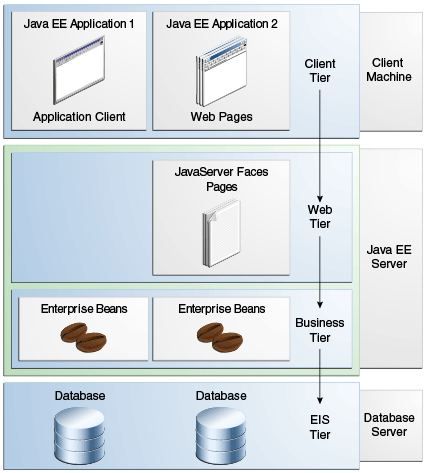
\includegraphics[width=0.75\textwidth]{multitiered_applications.png}
  \end{center}
  \fonte{adaptado de \citetext{javaee7}}
\end{figure}

% ---
\subsubsection{Camada Cliente}
% ---

Esta camada é composta de clientes aplicativos que acessam o servidor Java EE e que geralmente se localizam em máquinas diferentes da máquina do servidor:

\begin{itemize}
  \item Clientes Web - também chamados de \emph{clientes magros}, são compostos de páginas dinâmicas (\emph{e.g.}, XHTML) geradas na camada Web e por um navegador responsável por renderizá-las.
  \item Clientes Aplicativos - quando os usuários necessitam realizar atividades que requerem uma interface mais rica do que a disponibilizada por linguagens de marcação, utilizam-se clientes aplicativos baseados nas APIs Swing ou AWT (\emph{Abstract Window Toolkit})\footnote{Não obstante, pode-se utilizar uma interface em linha de comando.}. Embora seja possível o estabelecimento de uma conexão HTTP com um \emph{servlet} na camada Web, clientes aplicativos costumam acessar diretamente os \emph{beans} gerenciais da camada de negócio.
  \item \emph{Applets} - componentes embarcados que são incluídos nas páginas web. São escritos em Java e, portanto, necessitam da máquina virtual Java instalada no navegador web do cliente (e provavelmente do \emph{plugin} Java e de um arquivo de política de segurança).
\end{itemize}

% ---
\subsubsection{Camada Web}
% ---

É a camada responsável pela interação entre os clientes e a camada de negócios. Suas principais funções são:
\begin{itemize}
  \item Gerar, dinamicamente, conteúdo para o cliente em diversos formatos.
  \item Obter as entradas (dados e ações) da interface com o cliente e retornar os resultados dos componentes da camada de negócios.
  \item Controlar o fluxo das páginas no cliente.
  \item Manter o estado dos dados da sessão do usuário.
  \item Executar um pouco de lógica simples e armazenar dados em componentes JavaBeans temporariamente.
\end{itemize}

\emph{Servlets} e páginas web criadas com a tecnologia \emph{JavaServer Faces} (vide seção~\ref{sec:jsf}) são os componentes desta camada. \emph{Servlets} são classes Java que possuem métodos adequados a receber requisições e construir respostas às tais requisições dinamicamente. O trecho de código\cite{javaservlet} a seguir (vide \lstlistingname~\ref{alg:servlet}) representa um \texttt{HttpServlet}, que atende a requisições HTTP do tipo GET através da sobrescrita do método \texttt{doGet()}. Os parâmetros \texttt{HttpServletRequest} e \texttt{HttpServletResponse} representam, respectivamente, a requisição feita pelo cliente e a resposta do servidor.
%
\begin{lstlisting}[language=Java, caption={Um \emph{servlet} que imprime ``\emph{Hello World}''.}, label={alg:servlet}]
import java.io.*;
import javax.servlet.*;
import javax.servlet.http.*;

public class HelloWorld extends HttpServlet {
  public void doGet(HttpServletRequest req,
                    HttpServletResponse res)
      throws ServletException, IOException {
    res.setContentType("text/html");
    PrintWriter out = res.getWriter();
    out.println("<html>");
    out.println("<head><title>Hello World</title></head>");
    out.println("<body>");
    out.println("<big>Hello World</big>");
    out.println("</body></html>");
  }
}
\end{lstlisting}

Um \emph{servlet} HTTP pode, além do método \texttt{doGet()}, sobreescrever outros métodos, tais como \texttt{doPut()}, \texttt{doDelete()}, etc, que representam requisições HTTP do tipo PUT, DELETE, etc, respectivamente.


% ---
\subsubsection{Camada de Negócio}
% ---
A camada de negócios possui componentes que provêm a lógica do negócio da aplicação, ou seja, código que provê funcionalidades para um determinado domínio do negócio. As tecnologias utilizadas nessa camada são as seguintes:
\begin{itemize}
  \item Componentes Enterprise JavaBeans (EJB), que fornecem funcionalidades como gerenciamento de sessão, segurança, gerenciamento de transações, etc.
  \item \emph{Web services} (JAX-RS, JAX-WS).
  \item Entidades de persistência - Java Persistence API (JPA).
\end{itemize}


% ---
\subsubsection{Camada EIS}
% ---

A camada EIS consiste de servidores de bancos de dados, sistemas de planejamento de recursos empresariais e outras fontes de dados legados. Esses recursos geralmente se localizam em suas próprias máquinas e são acessados pela camada de negócios. As tecnologias utilizadas nessa camada são:
\begin{itemize}
  \item Java Database Connetivity API (JDBC) - uma interface que permite a conexão às bases de dados.
  \item Java Persistence API (JPA).
  \item Java Transaction API (JTA) - uma interface para a realização de transações.
\end{itemize}

% ---
\subsection{JavaServer Faces}\label{sec:jsf}
% ---

A tecnologia JavaServer Faces (JSF) é uma \emph{especificação} de uma API Java utilizada para a criação de interfaces de usuário em aplicações web. Com essa API, é possível:
%
\begin{itemize}
  \item Representar componentes e o gerenciamento dos seus estados;
  \item Fazer o controle de eventos;
  \item Realizar a validação e a conversão de dados no lado do servidor;
  \item Definir regras para a navegação entre páginas;
  \item Prover o suporte à internacionalização e acessibilidade;
\end{itemize}
%
Além da API, bibliotecas de \emph{tags} são utilizadas para adicionar os componentes às páginas web e para conectá-los aos objetos do servidor. Componentes, ou \emph{widgets}, são entidades autônomas e reutilizáveis da interface de usuário.

Existem duas implementações principais: Apache MyFaces e Oracle Mojarra. Ambas contêm pelo menos os componentes padrões, ou seja, os componentes responsáveis por gerar qualquer um dos elementos HTML básicos (tabelas, caixas de entrada de texto, botões, seletores, etc). Bibliotecas de componentes\footnote{Existem diversas bibliotecas disponíveis. As mais conhecidas são: PrimeFaces, RichFaces e ICEFaces.} oferecem funcionalidades previamente  testadas e eventualmente úteis, tais como tabelas capazes de ordenar, filtrar e selecionar linhas, organização do conteúdo em diversos tipos de painéis e menus, exibição de coleções em listas e árvores, etc, além da possibilidade de escolha de diversos temas (vide Figura~\ref{fig:primefaces_datatable}).

\begin{figure}[!ht]
  \caption{\label{fig:primefaces_datatable}Componente DataTable da biblioteca PrimeFaces. Evidencia-se o uso de um \emph{paginator} no topo da tabela e o uso do tema \emph{bluesky}.}
  \begin{center}
    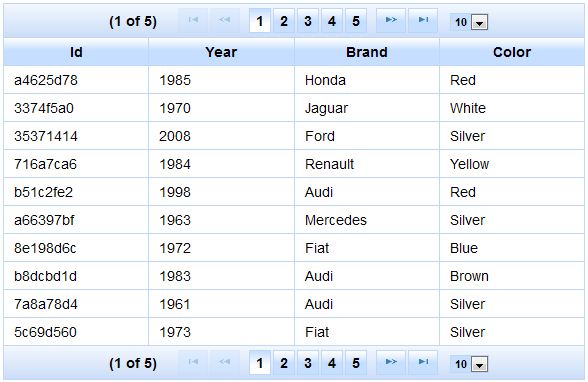
\includegraphics[width=0.75\textwidth]{/primefaces/datatable.png}
  \end{center}
  \fonte{PrimeFaces. Disponível em \url{https://www.primefaces.org/showcase/}}
\end{figure}

 
\subsubsection{Arquitetura do \emph{Framework}}

O \emph{framework} JSF segue o padrão arquitetural\footnote{Um padrão arquitetural expressa um esquema de organização estrutural para sistemas baseados em \emph{software}. O padrão provê um conjunto de subsistemas predefinidos, especifica suas responsabilidades, e inclui regras e diretrizes para organizar a relação entre eles.\cite{buschmann96}} MVC baseado em componentes. A grande vantagem desse padrão é a separação entre apresentação e comportamento (lógica) da aplicação:

\begin{description}
  \item[Visão] - fornece a representação da informação para o usuário da aplicação. Pode-se ter diversas visões do mesmo modelo. A tecnologia padrão utilizada pelo JSF é a Facelets (vide Seção~\ref{sec:facelets}).
  \item[Modelo] - representa o comportamento da aplicação em termos do domínio do problema, e independe da visão.
  \item[Controlador] - converte entradas/eventos em comandos para a visão ou para o modelo.
\end{description}

Todas as requisições feitas à aplicação devem passar primeiramente pelo controlador através do \texttt{FacesServlet}, que é o \emph{servlet} responsável por gerenciar o ciclo de vida do processamento de requisições. Ou seja, o próprio \emph{framework} JSF assume o papel de controlador no padrão MVC. Dessa forma, o desenvolvedor da aplicação não precisa se preocupar em escrever código \emph{boilerplate}\footnote{A implementação de diversos controladores para diferentes tipos de requisições é utilizada em \emph{action-based frameworks}, tais como o SpringMVC, Struts e ASP.NET.} tal como o do Algoritmo~\ref{alg:servlet}.

\begin{figure}[!ht]
  \caption{\label{fig:mvc}Comparação entre os dois tipos de padrão MVC. Em (A), tem-se o \emph{framework} baseado em componentes. Em (B), o baseado em ações. Os números ao lado das setas indicam a ordem do processamento de uma requisição.}
  \begin{center}
    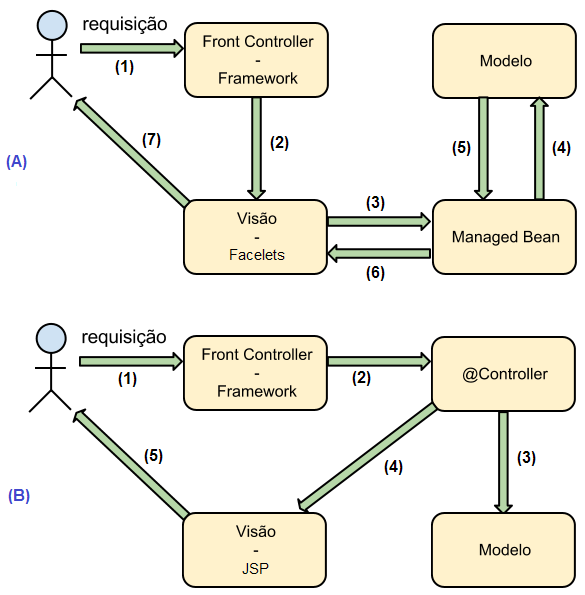
\includegraphics[width=0.75\textwidth]{/mvc/mvc.png}
  \end{center}
  \fonte{Caelum. Adaptado de \citetext{caelum}}
\end{figure}

%O JSF é dito ser um \emph{framework} baseado em componentes (ou \emph{MVC pull}) pelo fato de 

%
%Apenas testando:
%
%\begin{table}[!htb]
%  \IBGEtab{%
%    \caption{Um Exemplo de tabela alinhada que pode ser longa ou curta, conforme padrão IBGE.}%
%    \label{tabela-ibge}
%  }{%
%    \begin{tabular}{ccc}
%      \toprule
%      Nome & Nascimento & Documento \\
%      \midrule \midrule
%      Maria da Silva & 11/11/1111 & 111.111.111-11 \\
%      \bottomrule
%    \end{tabular}%
%  }{%
%    \fonte{Produzido pelos autores}%
%    \nota{Esta éuma nota, que diz que os dados são baseados na regressão linear.}%
%    \nota[Anotações]{Uma anotação adicional, seguida de várias outras.}%
%  }
%\end{table}


% ---
\subsection{Facelets}\label{sec:facelets}
% ---

% ---
\subsection{Primefaces}
% ---

% ---
\subsection{Java Persistence API}
% ---

% ---
\subsection{Hibernate}
% ---

% ---
\subsection{Spring}
% ---



\chapter{Análise e Projeto}
% ----------------------------------------------------------

% ---
\section{Módulo do Formulário de Inscrição}
% ---

% ---
\subsection{Elicitação e Análise de Requisitos}
% ---
% ---
\subsection{Diagramas de Classes}
% ---
% ---
\subsection{Diagramas de Casos de Uso}
% ---
% ---
\subsection{Diagramas de Atividades}
% ---
% ---
\subsection{Diagramas de Seqüência}
% ---
% ---
\subsection{Mock-Ups}
% ---

% ---
\section{Módulo Administrativo}
% ---

% ---
\subsection{Elicitação e Análise de Requisitos}
% ---
% ---
\subsection{Diagramas de Classes}
% ---
% ---
\subsection{Diagramas de Casos de Uso}
% ---
% ---
\subsection{Diagramas de Atividades}
% ---
% ---
\subsection{Diagramas de Seqüência}
% ---
% ---
\subsection{Mock-Ups}
% ---


\chapter{Implementação e Testes}
% ----------------------------------------------------------

% ---
\section{Testes de Unidade}
% ---

% ---
\section{Teste de Carga}
% ---



\chapter{Conclusões}
% ----------------------------------------------------------



% ----------------------------------------------------------
\bibliography{referencias}

%\begin{thebibliography}{9}
%
%\bibitem{lamport94}
%  Leslie Lamport,
%  \emph{\LaTeX: a document preparation system},
%  Addison Wesley, Massachusetts,
%  2nd edition,
%  1994.
%\end{thebibliography}


\end{document}
